\documentclass[12pt]{article}
\usepackage{amsmath}
\usepackage{fontspec}
\usepackage{lilyglyphs}
% \usepackage{musicography}
\usepackage{fourier}
\usepackage{float}

\floatstyle{ruled}
\newfloat{Example}{h}{example}[section]

% \setlength{\textheight}{8.5in} 
% \setlength{\textwidth}{6.35in}

\renewcommand{\sharp}{\lilyGlyph[scale=1.2,raise=.5]{accidentals.sharp}}
\renewcommand{\flat}{\lilyGlyph[scale=1.2,raise=.5]{accidentals.flat}}
\renewcommand{\natural}{\lilyGlyph[scale=1.2,raise=.5]{accidentals.natural}}
\renewcommand{\flatflat}{\lilyGlyph[scale=1.2,raise=.5]{accidentals.flatflat}}
\renewcommand{\doublesharp}{\lilyGlyph[scale=1.2,raise=.5]{accidentals.doublesharp}}

\newcommand{\mathscript}[1]{\text{\scriptsize #1}}
\newcommand{\fbtri}[3]{
    \begin{array}{l}
    \scriptstyle{#1}\\
    [-1.35ex]\scriptstyle{#2}\\
    [-1.35ex]\scriptstyle{#3}  
\end{array}
}

\title{An Example for Music Document}
\author{Yifei Wang}

\begin{document}
    \maketitle
    \section{Music symbols}
        The second inversion of a triad is denoted as $^6_4$, for example, V$^6_4$.The size of accidental notes is redefined. A\sharp. A\flat. A\natural. A\flat\flat. A\doublesharp. The E\flat\ major key is shown in Example. \ref{eg:Eflmajor}.
        \begin{Example}
            \caption{The E\flat\ major key}
            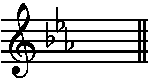
\includegraphics{Eflat-from-1.0.1-to-2.0.1-clip.pdf}
            \label{eg:Eflmajor}
        \end{Example}

        Note that the default size of accidentals provided by Lilyglyphs package so we have redefined them.

        I like the sudden change from \lilyDynamics{pp} to \lilyDynamics{ff}, which makes me excited. The dynamic \lilyDynamics{sf} is also good.

        Figured bass is also defined by us. We can write the figured bass in equations.
        \begin{equation*}
            \fbtri{7\mathscript{\flat}}{5}{3}
        \end{equation*}

        The size of Liliglyphs symbols cannot be modified in mathmode, so we define a `mathscript' command to switch to text mode and the apply the `scriptsize' command.

    \section{Example scores}

        In Example. \ref{eg:yanyuanqing} we show a piece of a song, Yan Yuan Qing, popular in Peking University. It is not the school song of Peking University, but students like it for it carries their love and responsibility for their home and country.
        \begin{Example}
            \caption{A song}
            \raggedright
            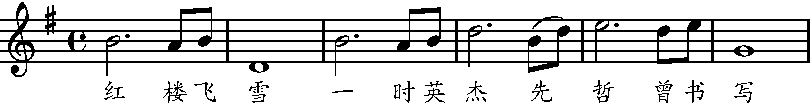
\includegraphics{yanyuanqing-from-1.0.1-to-17.0.1-clip-2.pdf}
            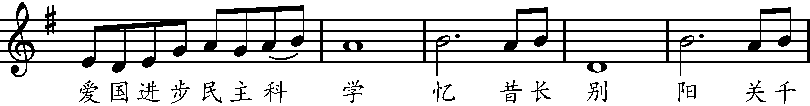
\includegraphics{yanyuanqing-from-1.0.1-to-17.0.1-clip-1.pdf}
            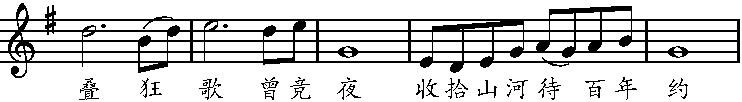
\includegraphics{yanyuanqing-from-1.0.1-to-17.0.1-clip.pdf}
            \label{eg:yanyuanqing}
        \end{Example}
        
\end{document}
